\documentclass{article}
\usepackage[utf8]{inputenc}

\title{GIF 4101 Rendu 1 Rapport Arnaud DALIE}
\author{Arnaud Dalié }
\date{September 2018}

\usepackage{natbib}
\usepackage{graphicx}

\begin{document}

\maketitle

\section{Introduction}
L'objectif de ce premier travail est de se familiariser avec les différentes méthodes paramétriques de base utilisées pour la classification.
Ce compte rendu a pour but de compléter les fichier $d1q2.py$ et $d1q2.py$ en détaillant les choix effectués, les améliorations possibles ainsi que de répondre aux différentes questions de l'énoncé.

\section{Travail à réaliser}

\subsection{Estimateurs statistiques}

Cette partie a pour but d'étudier l'estimateur $\lambda$ de la loi exponentielle grâce à la méthode du maximum de vraissemblace

a) On a :
$$
p(x) = \left\{
    \begin{array}{ll}
        \lambda exp(-\lambda x) \; x \in \left [ 0; \infty  \right [ \\
        0 \; x \in \left ] \infty ; 0  \right ]
    \end{array}
\right.
$$

On calcule la fonction de vraissemblace : 
$$
l(\lambda | X) = \prod_{i = 1}^{n} p(x_{i} | \lambda)
$$
On remarque que si ne serait-ce qu'une seule valeur de $X$ est négative, alors la vraissemblance tombe à $0$. C'est pourquoi on admettra que les valeurs de $X$ sont toutes positives.
$$
l(\lambda | X) = \prod_{i = 1}^{n} \lambda e^{\lambda x_{i}}
$$
Ensuite, on calcule la log-vraissemblance et on obtient :
$$
L(\lambda | X) = \sum_{i = 1}^{n} ln(\lambda) - \lambda x_{i}
$$
$$
L(\lambda | X) = nln(\lambda) - \lambda \sum_{i = 1}^{n} x_{i}
$$

On va chercher la valeure de $\lambda$ pourl aquelle cette valeure est maximale simplement en cherchant le point où la dérivée s'annule : 
$$
\frac{\partial L(\lambda | X)}{\partial \lambda} = \frac{n}{\lambda} - \sum_{i = 1}^{n} x_{i} 
$$
$$
\frac{\partial L(\lambda | X)}{\partial \lambda} = 0 \Leftrightarrow \frac{n}{\lambda} =\sum_{i = 1}^{n} x_{i} 
$$
$$
\Leftrightarrow \frac{1}{\lambda} = \frac{1}{n} \sum_{i = 1}^{n} x_{i} \\
$$
$$
\Leftrightarrow \lambda = \frac{1}{\bar{x}}
$$

On vérifie aisément que la dérivée seconde est négative pour tous $\lambda > 0$ et donc qu'on a bien à faire a un extremum qui est un maximum.\\

b) On va maintenant chercher à savoir si cet estiamteur est sans biais.
On cherche donc à vérifier :
$$
b_{\lambda}(\hat{\lambda}) = 0 
$$
$$
\Leftrightarrow \mathbb{E}_{X}\left [ \hat{\lambda}(X) \right ] - \lambda
\Leftrightarrow \mathbb{E}\left [ \frac{1}{\bar{x}} \right ] - \frac{1}{\mathbb{E}\left [ X \right ] } 
$$
$$
\Leftrightarrow \mathbb{E}\left [ \frac{1}{\bar{x}} \right ] = \frac{1}{\mathbb{E}\left [ \mathbb{E} \left [ X \right ] \right ] }
$$
$$
\Leftrightarrow \mathbb{E}\left [ \frac{1}{\bar{x}} \right ] = \frac{1}{\mathbb{E}\left [ \bar{x} \right ] }
$$

Or, on sait que :
$$
\mathbb{E}\left [ \frac{1}{x} \right ] \neq  \frac{1}{\mathbb{E}\left [ x \right ] }
$$

On peut donc conclure que l'estiamteur a bien un biais.

\subsection{Expérimentations avec scikit-learn}

Dans cette partie, on va tester les performances de dofférents classificateurs sur le jeu de données des Iris de Fisher. 

a) Voici les différentes variables mesurées par Fisher comparée deux à deux avec les classes représentées dans différentes couleurs. On remarque que les différentes sont facilement distingables pour les différents couples de variables étudiées, à l'exception de la classe verte et rouge dans le cas de la comparaison entre sepal width et sepal length (figure en haut à gauche). On constate également la nette séparation de la classe bleu avec les deux autres.

\begin{figure}[h!]
  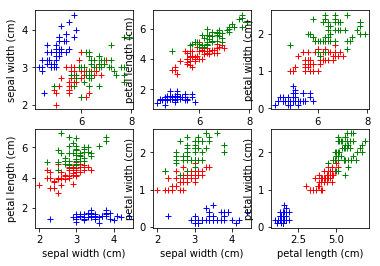
\includegraphics[width=\linewidth]{classes.png}
  \caption{Comparison of classes ratios between different variables}
  \label{fig:classes}
\end{figure}
\newpage
\newpage


b) On teste les différents classifieurs reposant sur l'Annalyse Discriminante Quadratique, l'Annalyse Discriminante Linéaire, la classification Bayesienne naïve et enfin la distance aux centroïdes.
Voici le tableau résumant les performances de chacuns pour les différents couples de variables. \\
% \usepackage{booktabs}
\begin{table}[h!]
\begin{tabular}{@{}llllll@{}}

        & Quadratic & Linear & Naïve Bayesian & Centroïd & Mean \\ 
SW / SL & 0.200     & 0.200  & 0.220          & 0.185    &      0.201 \\
PL / SL & 0.040     & 0.033  & 0.087          & 0.113    &      0.188\\
PW / SL & 0.033     & 0.040  & 0.040          & 0.060    &      0.043\\
PL / SW & 0.047     & 0.047  & 0.080          & 0.060    &      0.059\\
PW / SW & 0.047     & 0.033  & 0.053          & 0.060    &      0.048\\
PW / PL & 0.020     & 0.040  & 0.040          & 0.040    &      0.035
\end{tabular}
\end{table}

On remarque que les performances sont croissantes en fonction de la complexité du modèle. Avec ce jeu de données, on peut considérer le modèle des centroïdes comme un bon compromis entre performance et complexité ($\approx 90$\%). Il a, de manière surprenante, la meilleure performance pour le couple de variable qu'on avait considéré comme difficile à distinguer.

c) Pour cette question, on ne sépare plus les variables en couples. On fait directement l'entraînement et les tests sur les 4 variables à la fois. Cela rend la tâche plus facile pour le classifieur et on obtient pour les trois méthodes de test les resultats suivants : $err = 0.020$ quand on utilise le même ensemble d'apprentissage et de test, $err = 0.033$ pour l'utilisation de la moitié de l'ensemble pour l'apprentissage et enfin $err = 0.024$ pour la méthode à $k = 3$ plis.
On pouvait s'attendre à ces résultats. Le premier semble avoir la meilleur performance, mais on a surtout à faire à un $overfitting$ puisque les données utilisées pour apprendre le modèle sont les mêmes que pour le tester. Ensuite, on remarque que la méthode à $k = 3$ plis est plus performante que la seconde méthode. Pour une séparation en deux sous-ensembles égales, le modèle dispose de moins de données d'apprentissage que pour $k = 3$ dans la troisième méthode. On peut donc supposer qu'il y à un $k$ optimal pour avoir un maximum de données d'entraînement sans tomber dans l'overfitting.

d) On reteste les quatre classifieurs avec un jeu de données formant des cercles concentriques bien distinct. Comme on pouvait s'y attendre, les classifieurs linéaires comme LDA et NearestCentroids n'ont pas pu décider linéairement des classes et affichent donc des taux d'erreurs en moyenne de $50\%$ mais cependant très variables elon les conditions initiales. (Par exemple, vu que les deux centres sont quasiment identiques, python a du mal à calculer la pente de la frontière de décision et elle change donc à chaque execution. Ce calcul obéit sans doute à des lois d'arrondis et des approximations très bas niveau et hors du programme de ce cours)


\newpage
\subsection{Classement avec option de rejet}

Le but de cette dernière partie est l'implémentation d'un classificateur avec option de rejet. Avant de se lancer dans l'implémentation, il était demandé un petit exercice théorique consistant à calculer l'estimateur de $\sigma$ puis à expliciter la règle de décision avec rejet.

a) Les calculs suivent la même méthode que dans la partie 1.

$$
l(\sigma_{i}|X_{i}) = \prod_{t = 1}^{p} p(x_{i}^{t} |\sigma_{i}) 
$$
$$
= \prod_{t = 1}^{p} \frac{1}{\sqrt 2 \pi^{D}} \frac{1}{\sqrt det( \Sigma_{i} )}
e^{- \frac{1}{2} (x-\mu)^{T}\Sigma_{i}^{-1}(x-\mu)} 
$$
$$
= \prod_{t = 1}^{p} (2\pi)^{\frac{-N}{2}} det( \Sigma_{i} )^{- \frac{1}{2}} e^{- \frac{1}{2} (x-\mu)^{T}\Sigma_{i}^{-1}(x-\mu)} 
$$

La matrice $\Sigma$ étant de la forme $\sigma^{2} I$, on a :
$$
\Sigma_{i}^{-1} = \frac{1}{\sigma_{i}^{2}}I
$$
et :
$$
det(\Sigma_{i}) = \sigma{i}^{2D}  
$$

On obtient donc la log-vraissemblance suivante :

$$
L(X_{i}|\sigma_{i}) = \sum_{t=1}^{p} - \frac{D}{2}ln(2\pi) - Dln(\sigma_{i})-\frac{1}{2\sigma_{i}^{2}}\left \| x_{t} - \mu \right \|^{2} 
$$
$$
= -\frac{Dp}{2}ln(2\pi) - Dpln(\sigma_{i}) - \frac{1}{2\sigma_{i}^{2}}\sum_{t=1}^{p}\left \| x_{t} - \mu \right \|^{2}
$$

En dérivant : 
$$
\frac{\partial^2 L(X_{i}|\sigma_{i})}{\partial \sigma_{i}^2} = -\frac{Dp}{\sigma_{i}} + \frac{1}{\sigma_{i}^3}\sum_{t=1}^{p}\left \| x_{t} - \mu \right \|^{2}
$$

On cherche alors pour quelle valeur de $\sigma$  la dérivé s'annule :
$$
\frac{\partial^2 L(X_{i}|\sigma_{i})}{\partial \sigma_{i}^2} = 0 
$$
$$
\Leftrightarrow  \frac{Dp}{\sigma_{i}} = \frac{1}{\sigma_{i}^3}\sum_{t=1}^{p}\left \| x_{t} - \mu \right \|^{2} 
$$
$$
\Leftrightarrow \sigma_{i}^2 = \frac{1}{Dp}\sum_{t=1}^{p}\left \| x_{t} - \mu \right \|^{2} 
$$
$$
\Leftrightarrow \sigma_{i} = \sqrt{\frac{1}{Dp}\sum_{t=1}^{p}\left \| x_{t} - \mu \right \|^{2}}
$$

b) La probabilité à posteriori $P(C_{i}|X)$ peut donc être calculée. La formule développée est la suivante : 

$$
P(C_{i}|x) = \frac{P(C_{i}) * P(x|C_{i})}{P(x)} = \frac{P(C_{i}) * P(x|C_{i})}{\sum_{i = 1}^{N}P(C_{i}) * P(x|C_{i})} 
$$
$$
= \frac{\frac{P_{i}}{P} * 
\frac{1}{\sqrt {2\pi \sigma_{i}^{2D}}}e^{\frac{1}{2\sigma_{i}^{2}}\left \| x - \mu_{i}\right \|^{2}}
}{\sum_{j = 1}^{N}\frac{P_{j}}{P} * \frac{1}{\sqrt {2\pi \sigma_{j}^{2D}}}e^{\frac{1}{2\sigma_{j}^{2}}\left \| x - \mu_{j}\right \|^{2}}
}
$$
La fonction de perte s'écrit :

$$
\math L (c_{i}, C_{j}) = 
\left \{
\begin{array}
0 \> si \>  i=j 
\\ 
1 \> si \> i \neq j
\\
\lambda \> si\> i = K + 1
\end{array}

\right
$$

Le risque s'écrit alors comme suit pour les classes: 
$$
R(c_{i}|x) = \sum_{k = 1}^{K} L (c_{i}, C_{j})P(C_{k}|x)
= 1 - P(C_{i}|x) 
$$pour l'une des classes.
Et le risue de l'option de rejet s'écrit alors :
$$
R(c_{K + 1}|x) = \sum_{k = 1}^{K} \lambda P(C_{k}|x)
= \lambda
$$

En résolvant l'inéquation du risque, on obtient la fonction de prise décision minimisant le risque en fonction de $\lambda$ :
$$
c_{i} =
\left \{
\begin{array} {ll}
argmax_{C_{j} = C_{1}}^{C_{N}}(P(C_{j}|x)) \> si \> 
max(P(C_{j}|x)) > 1 -\lambda
\\ 
C_{N+1} \> sinon 
\end{array}
\right
$$

c) L'implémentation du classifieur ave coption de rejet se fait en quatres fonctions : \\
- fit : qui estime les différents paramètres du modèle pour chaque classe en fonction de l'ensemble donné. \\
- predict : qui calcule la probabilité de chaque classe en fonction des paramètres préalablement calculés. \\
- predict\_proba : qui applique la fonction de décision afin de choisir la classe prédite. \\
- score : qui appelle predic\_proba et retourne le taux de décision correctes.

d) Les performances pour les différents $\lambda$ sont les suivantes :

\begin{table}[h!]
\begin{tabular}{@{}llllll@{}}

\lambda        & 0.1   & 0.3   & 0.5   & 1     \\ 
SW / SL & 0.607 & 0.387 & 0.200 & 0.193 &      \\
PL / SL & 0.233 & 0.147 & 0.113 & 0.113 &      \\
PW / SL & 0.36  & 0.22  & 0.133 & 0.133 &      \\
PL / SW & 0.200 & 0.107 & 0.053 & 0.053 &      \\
PW / SW & 0.260 & 0.80  & 0.600 & 0.600 &      \\
PW / PL & 0.107 & 0.073 & 0.033 & 0.033 &     
\end{tabular}
\end{table}

A chaque fois, c'est le classifieur acceptant ne rejetant rien qui obtient le meilleur score. L'erreur est même décroissante avec l'augmentation de $\lambda$. On peut expliquer cela par le bon groupement et la bonne séparation des classes. En effet, les données sont bien regroupées et nes chevauchent quasiment pas (sauf pour une paire de variables). De fait, très peu de données ont des probabilités inférieures au seuil fixé par $lambda$. 

On peut conclure que dans les $\lambda$ choisis, aucun ne permet d'obtenir de resultats meilleurs sur notre dataset. Attention cependant, il se peut que sur de nouvelles données aberrantes ou plus bruitées, les régions de rejet soit plus déterminantes.   

\end{document}
